\section{Лекция номер 5}
\subsection{Знакопостоянные ряды}
Мы можем считать, что члены ряда неотрицательны, ведь в ином случае просто поменяем знак у них всех.

\begin{theorem}
    Если $a_n \geqslant 0$, то ряд сходится, если и только если его частичные суммы ограничены сверху.
\end{theorem}
\begin{proof}
    Обозначим за $S_n := \sum\limits_{k=1}^n a_k$. 
    Тогда по определению ряд сходится $\Leftrightarrow$ $S_n$ имеют конечный предел.
    Заметим, что $S_n$ момнотонно возрастает, так как члены ряда неотрицательны, значит по т. Вейерштрасса $S_n$ имеет предел $\Leftrightarrow$ она ограничена сверху.
\end{proof}

\vspace{4mm}

\textbf{Признак сравнения.} 
Пусть $0 \leqslant a_n \leqslant b_n$. 
Тогда \begin{enumerate}
    \item Если $\sum b_n$ сходится, то $\sum a_n$ тоже сходится.
    \item Если $\sum a_n$ расходится, то $\sum b_n$ тоже расходится.
\end{enumerate}
Можно считать, что неравенство выполняется лишь с некоторого момента, так как отбрасывание конечного префикса на сходимость не влияет.
\begin{proof}
    Заведем частичные суммы $A_n := \sum\limits_{k=1}^n a_k, B_n = \sum\limits_{k=1}^n b_k$.
    Очевидно, что $A_n \leqslant B_n$.
    Теперь просто воспользуемся предыдущей теоремой для доказательства каждого пункта:
    \begin{enumerate}
        \item $\sum b_n$ сходится $\Rightarrow B_n$ ограниены сверху $\Rightarrow A_n$ ограничены сверху $\Rightarrow \sum a_n$ сходится. 
        \item От противного: $\sum b_n$ сходится $\Rightarrow \sum a_n$ сходится по первому пункту. Противоречие. 
    \end{enumerate}
\end{proof}

\begin{follow}
    \begin{enumerate}
        \item Если $a_n, b_n \geqslant 0, a_n = O(b_n)$ и $\sum b_n$ сходится, то $\sum a_n$ сходится. 
        \item Если $a_n \thicksim b_n$, то $\sum a_n$ и $\sum b_n$ ведут себя одинаково.
    \end{enumerate}
    Понятно, что все это при $n \to +\infty$.
\end{follow}
\begin{proof} \quad 

    \begin{enumerate}
        \item По условию $0 \leqslant a_n \leqslant cb_n$, а мы знаем, что $\sum cb_n$ сходится, так как константу мы можем заносить, тогда по признаку сравнения $\sum a_n$ сходится.
        \item $a_n \thicksim b_n \Rightarrow \lim \frac{a_n}{b_n} = 1 \Rightarrow \frac{1}{2} \leqslant \frac{a_n}{b_n} \leqslant 2$ при больших $n$.
    
        Отсюда следуют 2 неравенства: $\begin{cases}
            a_n \leqslant 2b_n \\
            b_n \leqslant 2a_n
        \end{cases}$ при больших $n$. Тогда по признаку сравнения они ведут себя одинаково.
    \end{enumerate}
\end{proof}

\vspace{4mm}

\textbf{Признак Коши.} 
Пусть $a_n \geqslant 0$. Тогда:
\begin{enumerate}
    \item Если $\sqrt[n]{a_n} \leqslant q < 1$, то ряд сходится.
    \item Если $\sqrt[n]{a_n} \geqslant 1$, то ряд расходится.
    \item Пусть $q^* := \overline{\lim}_{n \to \infty} \sqrt[n]{a_n}$.
    Если $q^* < 1$, то ряд сходится, если $q^* > 1$, то ряд расходится, иначе ничего утверждать нельзя.
\end{enumerate}
\begin{proof} \quad

    \begin{enumerate}
        \item $a_n \leqslant q^n$ при $q < 1 \Rightarrow$ применяем признак сравнения с бесконечно убывающей геометрической прогрессией.
        \item $a_n \geqslant 1$, нет необходимого условия сходимости.
        \item Пусть $q^* > 1$. 
        Вспомним, что это наибольший частичный предел и возьмем эту подпоследовательность: $\sqrt[n_k]{a_{n_k}} \to q* > 1$.
        Тогда $\sqrt[n_k]{a_{n_k}} > 1$ при больших $k$ $\Rightarrow a_{n_k} > 1$ при больших $k$.
        Опять не выполняется необходимое условие сходимости.

        Пусть $q^* < 1$. 
        Распишем верхний предел по определению: $q^* = \lim\limits_{n \to \infty} \sup\limits_{k \geqslant n} \sqrt[k]{a_k} < 1$. 
        Значит, с какого-то момента $\sup\limits_{k \geqslant n} \sqrt[k]{a_k} < \frac{q^* + 1}{2}$ (это середина отрезка от $q^*$ до 1).
        Супремум не меньше членов подпоследовательности, поэтому $\sqrt[n]{a_n} < \frac{q^* + 1}{2} < 1$ с какого-то момента.
        Осталось применить первый пункт.
    \end{enumerate}
\end{proof}

\underline{Примеры, когда $q^* = 1:$}
\begin{enumerate}
    \item У гармонического ряда $q^* = 1$, а он расходится.
    \item У ряда $\sum\limits_{n=1}^{\infty} \frac{1}{n(n+1)}$ $q^*$ тоже равен 1, но он сходится. 
\end{enumerate}

\vspace{15mm}

\textbf{Признак Даламбера:} 
Пусть $a_n > 0$. Тогда: \begin{enumerate}
    \item Если $\frac{a_{n+1}}{a_n} \leqslant d < 1$, то $\sum a_n$ сходится.
    \item Если $\frac{a_{n+1}}{a_n} \geqslant 1$, то $\sum a_n$ расходится.
    \item Пусть $d^* := \lim\limits_{n \to \infty} \frac{a_{n+1}}{a_n}$. Если $d^* < 1$, то ряд сходится, если $d^* > 1$, то расходится, иначе ничего утверждать нельзя (примеры те же).
\end{enumerate}
\begin{proof} \quad

    \begin{enumerate}
        \item В этом пункте утверждается, что $a_{n+1} \leqslant da_n \leqslant d^2a_{n - 1} \leqslant \dots \leqslant d^na_1$. Применяем признак сравнения с бесконечно убывающей геометрической прогрессией.
        \item В этом пункте $a_{n+1} \geqslant a_n$, значит, нет необходимого условия сходимости.
        \item Пусть $d^* < 1$. Вспомним, что это $\lim\limits_{n \to \infty} \frac{a_{n+1}}{a_n}$, а значит с какого-то момента $\frac{a_{n+1}}{a_n} < \frac{d^* + 1}{2} < 1$. Осталось применить первый пункт.
        
        Пусть $d^* > 1$. Тогда с какого-то момента $\frac{a_{n+1}}{a_n} \geqslant 1$. Осталось применить второй пункт.
    \end{enumerate}
\end{proof}

\begin{example}
    Исследуем на сходимость ряд $\sum\limits_{n = 1}^\infty \frac{x_n}{n!}$ при $x > 0$.

    По Даламберу: $\frac{a_{n+1}}{a_n} = \frac{x^{n+1}n!}{(n+1)!x^n} = \frac{x}{n+1} \to 0 \Rightarrow$ ряд сходится.

    По Коши: $\sqrt[n]{a_n} = \frac{x}{\sqrt[n]{n!}} \thicksim \frac{x}{\sqrt[n]{n^ne^{-n}\sqrt{2\pi n}}} = \frac{x}{ne^{-1}\sqrt[2n]{2\pi n}} \to 0 \Rightarrow$ ряд сходится.
\end{example}

\vspace{5mm}


\begin{theorem} (связь пр. Коши и Даламбера)
    Если $a_n > 0$ и $d^* = \lim\limits_{n \to \infty} \frac{a_{n+1}}{a_n}$, то  = $\lim\limits_{n \to \infty} \sqrt[n]{a_n} = d^*$.
\end{theorem}
\begin{proof}
    Будем считать $\lim\limits_{n \to \infty} \ln(\sqrt[n]{a_n}) = \lim\limits_{n \to \infty} \frac{\ln a_n}{n}$.
    Для этого применим т. Штольца (знаменатель строго возрастает и стремится в $+\infty$): \[ \lim\limits_{n \to \infty} \frac{\ln a_n}{n} = \lim\limits_{n \to \infty} \frac{\ln a_{n+1} - \ln a_n}{n + 1 - n} = \lim\limits_{n \to \infty} \ln \frac{a_{n+1}}{a_n} = \ln d^* \]
    \quad Значит, $\lim\limits_{n \to \infty} \sqrt[n]{a_n} = e^{\ln d^*} = d^*$
\end{proof}

\vspace{6mm}

\begin{theorem} (связь между суммами и интегралами)

    \quad Пусть $f: [a, b] \to \R$ монотонна. Тогда \[ \left| \sum_{k = a}^b f(k) - \int_a^b f(x)dx \right| \leqslant \max\{|f(a)|, |f(b)| \}\] 
\end{theorem}
\begin{proof}
    Пусть $f$ монотонно убывает и $f \geqslant 0$.
    Посмотрим на 2 суммы: \[ \sum\limits_{k = a}^{b-1} f(k) \geqslant \int_a^b f(x)dx \geqslant \sum\limits_{k = a + 1}^b f(k) \]
    \begin{center}
        %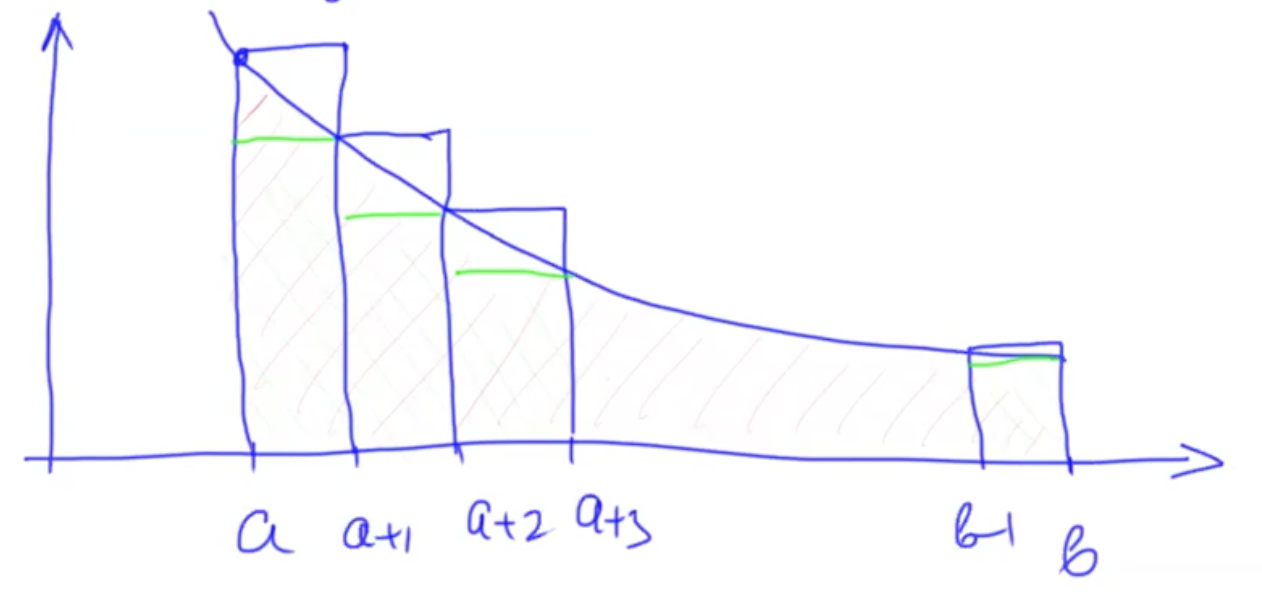
\includegraphics[scale=0.5]{images/lec5_pic1.png}
        \begin{tikzpicture}[thick,yscale=0.8]
            % Axes
            \draw[-latex,name path=xaxis] (-1,0) -- (10,0) node[above]{};
            \draw[-latex] (0,-2) -- (0,8) node[right]{};
            
            % Function plot
            \draw[ultra thick, orange,name path=function]  plot[smooth,domain=1.2:8] (\x, {1/(0.2*\x-0.1) + 0.6}) node{};

            % Draw columns
            \draw[ultra thick, violet, name path=0function] (1.5, 0) -- (1.5, 5.5) node[circle,fill,inner sep=1pt]{};
            \draw[ultra thick, violet, name path=1function] (2.5, 0) -- (2.5, 5.5);
            \draw[ultra thick, violet] (1.5, 5.5) -- (2.528, 5.5);

            \draw [ultra thick, pink, name intersections={of=function and 1function}] ($(intersection-1)+(0.028,0)$) -- ++(-1,0);
            \draw [ultra thick, violet, name intersections={of=function and 1function}] ($(intersection-1)-(0.028,0)$) -- ++(1.056,0);
            \draw [ultra thick, violet, name intersections={of=function and 1function}, name path=2function] ($(intersection-1)+(1,0)$) -- ++(0,-3.1);

            \draw [ultra thick, pink, name intersections={of=function and 2function}] ($(intersection-1)+(0.028,0)$) -- ++(-1,0);
            \draw [ultra thick, violet, name intersections={of=function and 2function}] ($(intersection-1)-(0.028,0)$) -- ++(1.056,0);
            \draw [ultra thick, violet, name intersections={of=function and 2function}, name path=3function] ($(intersection-1)+(1,0)$) -- ++(0,-2.26);

            \draw [ultra thick, pink, name intersections={of=function and 3function}] ($(intersection-1)-(0.028,0)$) -- ++(-0.944,0);

            \draw[ultra thick, violet, name path=5function] (7, 0) -- (7, 1.4);
            \draw[ultra thick, violet, name path=4function] (8, 0) -- (8, 1.4);
            \draw[ultra thick, violet] (6.972, 1.4) -- (8.028, 1.4);
            \draw[ultra thick, pink] (7.028, 1.25) -- (7.972, 1.25);
            
            % % x-axis labels
            \draw [name intersections={of=0function and xaxis}] ($(intersection-1)+(0,0.1)$) -- ++(0,-0.2) node[below] {\small $a$} ;
            \draw [name intersections={of=1function and xaxis}] ($(intersection-1)+(0,0.1)$) -- ++(0,-0.2) node[below] {\small $a+1$} ;
            \draw [name intersections={of=2function and xaxis}] ($(intersection-1)+(0,0.1)$) -- ++(0,-0.2) node[below] {\small $a+2$} ;
            \draw [name intersections={of=3function and xaxis}] ($(intersection-1)+(1,0.1)$) -- ++(0,-0.2) node[below] {\small $a+3$} ;
            \draw [name intersections={of=5function and xaxis}] ($(intersection-1)+(0,0.1)$) -- ++(0,-0.2) node[below] {\small $b-1$} ;
            \draw [name intersections={of=4function and xaxis}] ($(intersection-1)+(0,0.1)$) -- ++(0,-0.2) node[below] {\small $b$} ;
        \end{tikzpicture}
    \end{center}
    \quad Случай, когда $f$ не обязательно неотрицательна, сводится к этому прибавлением константы.
    Действительно, сделаем функцию неотрицательной прибавлением константы $c$, тогда как суммы, так и интеграл изменятся на $+c(b - a)$, то есть неравенство сохранится.

    \quad Теперь вычтем из неравенства всю сумму: \[ -f(b) \geqslant \int_a^b f(x)dx - \sum\limits_{k = a}^b f(k) \geqslant -f(a) \]
    \quad Добавив модуль, получаем искомое неравенство.

    \quad Случай, когда $f$ монотонно возрастает рассматривается аналогично.
\end{proof}

\vspace{6mm}

\textbf{Интегральный признак.}
Пусть $f: [1, +\infty) \to [0, +\infty)$ монотонна. 
Тогда $\sum\limits_{n = 1}^\infty f(n)$ и $\int_1^{+\infty} f(x)dx$ ведут себя одинаково. 
\begin{proof}
    Если $f$ монотонно возрастает, то, очевидно, и то, и то расходится.
    Пусть $f$ монотонно убывает. 
    Члены ряда неотрицательны, поэтому его сходимость равносильна ограниченности частичных сумм $S_n := \sum\limits_{k = 1}^n f(k)$.
    Сходимость же интеграла равносильна ограниченности первообразной $F(x) := \int_1^x f(x)dx$.  
    Чтобы связать эти ограниченности воспользуемся теоремой: \[ \left| S_n - F(n) \right| \leqslant f(1) (\text{не рассматриваем $f(n)$ так как $f$ убывает}) \]
    \quad Значит, ограниченность $S_n \Leftrightarrow$ ограниченность $F(n)$.
    
    \quad Но мы брали первообразную только в натуральных точках, значит, нам надо еще понять, что ограниченность $F(n) \Leftrightarrow$ ограниченность $F(x)$.
    Это очевидно, так как из-за неотрицательности $f$ первообразная $F$ монотонно возрастает, а значит, $F(x) \leqslant F(n)$ при $x \leqslant n$.

    \quad Таким образом, мы показали, что ограниченность $S_n \Leftrightarrow$ ограниченность $F(x)$. 
    Следовательно, мы показали равносильность сходимости суммы и интеграла.
\end{proof}

\vspace{6mm}

\begin{example}
    Установим, при каких $p$ сходится ряд $\sum\limits_{n = 1}^{\infty} \frac{1}{n^p}$.
    При $p \leqslant 0$, ряд очевидно расходится. 
    Пусть $p > 0$.
    Введем функцию $f(x) = \frac{1}{x^p}$, которая неотрицательна и монотонно убывает. 
    Тогда согласно интегральному признаку $\sum\limits_{n = 1}^{\infty} \frac{1}{n^p}$ и $\int_1^{+\infty} \frac{dx}{x^p}$ ведут себя одинаково. 
    А про интеграл мы уже все знаем, он сходится, когда $p > 1$. 
    Следовательно, $\sum\limits_{n = 1}^{\infty} \frac{1}{n^p}$ сходится при $p > 1$.
\end{example}

\begin{follow}
    С таким рядом удобно писать признак сравнения: если $0 \leqslant a_n \leqslant \frac{c}{p^n}$ при $p > 1$, то $\sum a_n$ сходится. 
\end{follow}

\begin{example}
    Исследуем на сходимость ряд $\sum\limits_{n = 2}^\infty \frac{1}{n\ln n}$. 
    Введем функцию $f(x) = \frac{1}{x\ln x}$. Она $> 0$ и монотонно убывает $\Rightarrow$ интегральный признак: \[ \int_2^{+\infty} \frac{dx}{x\ln x} = \ln(\ln x)\big|_2^{+\infty} = +\infty \]
    Значит, ряд расходится. 
\end{example}

\subsection{Знакоперменные ряды}
\textbf{Преобразование Абеля.} (дискретный аналог интегрирования по частям) \[ \sum_{k = 1}^n a_kb_k = A_nb_n + \sum_{k = 1}^{n - 1} A_k(b_k - b_{k+1}), \] где $A_k = a_1 + \dots + a_k$, считая $A_0 = 0$.
\begin{proof}
    \begin{gather*}
        \begin{split}
            \sum_{k = 1}^n a_kb_k &= \sum_{k = 1}^n (A_k - A_{k-1})b_k \\
            &= \sum_{k = 1}^n A_kb_k - \sum_{k = 1}^n A_{k-1}b_k \text{ (разделили на 2 суммы)} \\
            &= A_nb_n + \sum_{k = 1}^{n-1} A_kb_k - \sum_{k = 2}^n A_{k-1}b_k \text{ (вынесли одно слагаемое и убрали $A_0 = 0$)} \\
            &= A_nb_n + \sum_{k = 1}^{n-1} A_kb_k - \sum_{j = 1}^{n-1} A_jb_{j+1} \text{ (сменили переменную)} \\
            &= A_nb_n + \sum_{k = 1}^{n-1} A_k(b_k - b_{k+1}) \text{ ($j$ и $k$ пробегают одни и те же индексы)} \\
        \end{split}
    \end{gather*}
\end{proof} 

\textbf{Признак Дирихле.} 

 Пусть \begin{enumerate}
    \item $A_n := \sum\limits_{k = 1}^n a_k$ ограничены
    \item $b_n$ монотонно стремится к 0
\end{enumerate}
Тогда $\sum a_nb_n$ сходится.
\begin{proof}
    Применим преобразование Абеля: $S_n := \sum\limits_{k=1}^n a_kb_k = A_nb_n + \sum\limits_{k=1}^{n-1} A_k(b_k - b_{k+1})$.
    \quad Надо доказать, что существует конечный $\lim S_n$, т.е. конечные $\lim\limits_{n \to \infty} A_nb_n$ и $\lim\limits_{n \to \infty} \sum\limits_{k=1}^{n-1} A_k(b_k - b_{k+1})$.
    С первым пределом все понятно, так как $A_n$ ограничены, а $b_n \to 0$.
    Существование второго предела равносильно сходимости ряда $\sum\limits_{k=1}^{\infty} A_k(b_k - b_{k+1})$.

    \quad Докажем, что он сходится абсолютно. 
    По условию $|A_n| \leqslant M$, а $b_n$ монотонно стремятся к 0, причем будем считать, что они убывают (если возрастают, поменяем знкаки).
    Тогда \[ |A_k(b_k - b_{k+1})| \leqslant M|b_k - b_{k+1}| = M(b_k - b_{k+1}) \]
    \quad То есть мы можем ограничить таким рядом: $ \sum\limits_{k=1}^{\infty} M(b_k - b_{k+1}) = M\sum\limits_{k=1}^{\infty} (b_k - b_{k+1}) $. 
    Его частичная сумма это телескопическая сумма, после сокращения получаем $\sum\limits_{k=1}^{n} = b_1 - b_{n+1} \to b_1$.
    Следовательно, $M\sum\limits_{k=1}^{\infty} (b_k - b_{k+1}) = Mb_1$, то есть он сходится, а значит сходится и наш ряд по признаку сравнения.
\end{proof}

\vspace{6mm}

\textbf{Признак Абеля.} 

Пусть \begin{enumerate}
    \item $\sum\limits_{n=1}^\infty a_n$ сходится
    \item $b_n$ монотонны и ограничены
\end{enumerate}
Тогда $\sum\limits_{n=1}^\infty a_nb_n$ сходится.
\begin{proof}
    Второе и третье условие говорят нам о том, что существует конечный $\lim\limits_{n \to \infty} b_n = b$.
    Тогда $\widetilde{b}_n := b_n - b$ монотонно стремится к 0.

    \quad Первое условие говорит нам о том, что частичные суммы $A_n$ имеют конечный предел, следовательно, ограничены.
    Тогда $\sum\limits_{n=1}^\infty a_n\widetilde{b}_n$ сходится по Дирихле.

    \quad Используя полученное, перепишем наш ряд следующим образом: \[ \sum_{n=1}^\infty a_nb_n = \sum_{n=1}^\infty a_n(\widetilde{b}_n + b) = \underbrace{\sum_{n=1}^\infty a_n\widetilde{b}_n}_{\text{пр. Дирихле}} + \underbrace{b\sum_{n=1}^\infty a_n}_{\text{сх-ся по усл.}} \]
    \quad Таким образом, $\sum\limits_{n=1}^\infty a_nb_n$ сходится.
\end{proof}

\vspace{4mm}

\begin{example}
    Исследуем на сходимость $\sum\limits_{n=1}^\infty \frac{\sin n}{n^p}$.
    \begin{itemize}
        \item Если $p > 1$, то ряд сходится абсолютно, ведь $\frac{|\sin n|}{n^p} \leqslant \frac{1}{n^p}$.
        \item Если $0 < p \leqslant 1$, то будем применять признак Дирихле: $a_n = \sin n, b_n = \frac{1}{n^p}$. 
        Частичные суммы $A_n$ действительно ограничены, так как $A_n = \sum\limits_{k=1}^n \sin k = \frac{\sin \frac{n+1}{2}\sin \frac{n}{2}}{\sin \frac{1}{2}}$. Тогда по признаку Дирихле ряд сходится.
        \item Если $p \leqslant 0$, то $\lim \frac{\sin n}{n^p} \neq 0$, так как $\sin n \nrightarrow 0$. Необходимое условие невыполнено, ряд расходится.
        \item Также заметим, что при $0 < p \leqslant 1$ ряд $\frac{|\sin n|}{n^p}$ расходится, так как либо $|\sin n| \geqslant \sin \frac{1}{2}$, либо $|\sin (n+1)| \geqslant \sin \frac{1}{2}$.
    \end{itemize}
\end{example}

\vspace{8mm}

Отдельного внимания заслуживают знакочередующиеся ряды.
\begin{conj}
    Знакочередующийся ряд -- это ряд вида $\sum\limits_{n=1}^\infty (-1)^{(n-1)}a_n$, где $a_n \geqslant 0$.
\end{conj}

\textbf{Признак Лейбница.} Если $a_n$ монотонны и $\lim a_n = 0$, то $\sum\limits_{n=1}^\infty (-1)^{(n-1)}a_n$ сходится.
Более того, его сумма зажата между четными и нечетными частичными суммами: $S_{2n} \leqslant S \leqslant S_{2n + 1}$.

\begin{proof}
    Посмотрим на четные и нечетные частичные суммы: \begin{itemize}
        \item $S_{2n + 2} = S_{2n} + a_{2n + 1} - a_{2n + 2} \geqslant  S_{2n}$, так как $a_n$ монотонно убывает.
        \item $S_{2n + 1} = S_{2n - 1} - a_{2n} + a_{2n + 1} \leqslant S_{2n - 1}$, так как $a_n$ монотонно убывает.
    \end{itemize}
    \quad Получили последовательность вложенных отрезков: \[ [0, S_1] \supset [S_2, S_3] \supset [S_4, S_5] \supset \dots \]
    \quad На самом деле, это даже стягивающиеся отрезки, так как $\lim (S_{2n+1} - S_{2n}) = \lim a_{2n+1} = 0$.
    Тогда есть единственная общая точка $S$ такая, что $\lim S_{2n} = S = \lim S_{2n+1} \Rightarrow \lim S_n = S$ и $S \in [S_{2n}, S_{2n+1}] \Rightarrow S_{2n} \leqslant S \leqslant S_{2n+1}$.
\end{proof}

\begin{example}
    Исследуем на сходимость $\sum\limits_{n=1}^\infty \frac{(-1)^{n-1}}{n^p}$:
    \begin{itemize}
        \item При $p > 0$ ряд сходится по признаку Лейбница, так как $a_n = \frac{1}{n^p}$ монотонно $\to 0$.
        \item При $p \leqslant 0$ получаем, что $\frac{(-1)^{n-1}}{n^p} \nrightarrow 0$, и ряд расходится.
        \item При $p = 1$ получаем так называемый ряд Лейбница -- $\sum\limits_{n = 1}^\infty \frac{(-1)^{n-1}}{n}$. Найдем его сумму:
        \begin{gather*}
            \begin{split}
                S_{2n} &= 1 - \frac{1}{2} + \frac{1}{3} - \frac{1}{4} + \dots - \frac{1}{2n} \\
                &= 1 + \frac{1}{2} + \frac{1}{3} + \dots + \frac{1}{2n} - 2(\frac{1}{2} + \frac{1}{4} + \dots + \frac{1}{2n}) \\
                &= H_{2n} - H_n = \ln 2n + \gamma + o(1) - (\ln n + \gamma + o(1)) = \ln 2 + o(1)
            \end{split}
        \end{gather*}
        Отсюда делаем вывод, что $\sum\limits_{n = 1}^\infty \frac{(-1)^{n-1}}{n} = \ln 2$.
        
        Теперь переставим элементы и попробуем найти сумму получившегося ряда: \[ 1 - \frac{1}{2} - \frac{1}{4} + \frac{1}{3} - \frac{1}{6} - \frac{1}{8} + \frac{1}{5} - \frac{1}{10} - \frac{1}{12} + \dots \]
        \begin{gather*}
            \widetilde{S}_{3n} = \sum_{k = 1}^n \left(\underbrace{\frac{1}{2k - 1} - \frac{1}{2(2k - 1)}}_{= \frac{1}{2(2k - 1)}} - \frac{1}{2 * 2k}\right) = \\ 
            =  \frac{1}{2}\sum_{k = 1}^n \left(\frac{1}{2k - 1} - \frac{1}{2k}\right) = \frac{1}{2}\left(1 - \frac{1}{2} + \frac{1}{3} - \frac{1}{4} + \dots - \frac{1}{2n}\right) = \frac{S_{2n}}{2} \\
            \Rightarrow \widetilde{S}_{3n} \to \frac{\ln 2}{2}
        \end{gather*}
        
    \end{itemize}
\end{example}